\documentclass[a4paper, 12pt]{scrartcl}



\usepackage[utf8]{inputenc}

\usepackage[ngerman]{babel}
\usepackage{amssymb}
\usepackage[T1]{fontenc}
\usepackage{mathtools}
\usepackage{amsmath}
\usepackage{ntheorem}
\usepackage{bbm}
\usepackage{dsfont}
\usepackage{color}
\usepackage{slashed}
\usepackage{hyperref}
\usepackage{graphicx} 
\usepackage{bm}
\usepackage{mathabx}
\usepackage{float}
\usepackage{mwe}
\usepackage{multirow}
\begin{document}
\begin{titlepage}
	\centering
	{\scshape\LARGE Universität Tübingen \par}
	\vspace{2cm}
	{\huge\bfseries Franck-Hertz Versuch \par}
	\vspace{2cm}
	{\Large \scshape Blockpraktikum 2021} \par
	\vspace{2cm}
	{\Large  Erste korrigierte Version} \par
	\vspace{2cm}
	{\Large\itshape \underline{David Schütz} \space \space  \underline{Christian Gommeringer}\par}
	\vfill 
	{\large unter Betreuung von Alexander Göggelmann }
	\vfill

	{\large \today\par}
\end{titlepage}
\newpage 
\tableofcontents 

\newpage
\section{Einleitung}
\begin{flushleft}
Der Frank-Hertz Versuch hat historische Bedeutung, da es im zum ersten Mal gelungen ist, zu zeigen, dass Elektronen in einem Atom nur diskrete Energiepositionen einnehmen können. Damit unterstützte er die Aussagen des Bohrschen Atommodells.



\end{flushleft}
% | > <
\section{Theoretische Grundlagen} 

Heute wissen wir durch die Quantenmechanik bestätigt, dass Atome wirklich nur bestimmte diskrete Energien besitzen. Es ist möglich ein Atom in einen höheren Energiezustand anzuregen. Dabei verändert sich die Aufenthaltswahrscheinlichkeit des Elektrons und theoretisch auch des Atomkerns. Die gehen aber gewöhnlich nach kurzer Zeit in einen niederen Zustand über und senden dabei elektromagnetische Strahlung aus. Bei diesem Prozess sind allerdings nur bestimmte Übergänge möglich, die über die sogenannten Auswahlregeln festgelegt sind. Wichtig ist dass im an diesem Prozess beteiligten System Energieerhaltung und Drehimpulserhaltung eingehalten werden.
Beim Wasserstoffatom gibt es diese Energieniveaus 
\begin{equation*}E_n=-Ry\,\frac{1}{n^2}\end{equation*}
mit der Rydberg Konstante $Ry=13.6\,eV$. Die Energie, um ein Atom anzuregen, kann von außen zum Beispiel ein Elektron sein das unelastisch mit diesem Atom stößt, wie es bei diesem Versuch der Fall ist.
Ich möchte noch kurz das Bohrsche Atommodell vorstellen, da es historisch im Zusammenhang mit diesem Versuch bedeutend ist. Im Bohrschen Atommodell besteht das Atom aus einem Kern und Elektronen, die auf klassischen Bahnen um diesen Kern kreisen. Allerdings sind nicht alle klassischen Bahnen erlaubt. sondern nur bestimmte Bahnen. Auf diesen Bahnen emittiert das Elektron keine Energie, wie die Elektrodynamik eigentlich vorschreibt. Es ist möglich, dass ein Elektron von einer erlaubten Bahn auf eine andere springt. Dabei emittiert es die entstandene Energiedifferenz im Atom als elektromagnetische Strahlung. Deren Frequenz ist allerdings nicht durch die Umlauffrequenz erzeugt sondern über die Beziehung $f=\Delta{E}/h$ von der Energiedifferenz $\Delta{E}$. Durch ein weiteres Postulat wird zusätzlich die Bedingung, dass der Drehimpuls des Atoms nur vielfache Werte von $\bar{h}$ annehmen kann, erhalten.


\section{Versuchsaufbau und Durchführung}
In diesem Versuch untersuchen wir die Anregungsenergien des Neon Atoms und können daraus die Energieniveaus ableiten. Aus einer Glühkathode werden Elektronen herausgelöst und durch ein Beschleunigungsspannung beschleunigt um auf Neonatome zu treffen und mit diesen zu stoßen. Sie können elastisch und unelastisch mit ihnen stoßen, letzteres indem sie das Atom in einen anderen Energiezustand anregen. Das Experiment wird so durchgeführt, dass die Beschleunigungsspannung kontinuierlich erhöht wird und hinter dem Bereich, in dem die Streuung stattfindet, ein Detektor angebracht wird, der das Auftreffen eines Elektrons registriert. Am Detektor liegt noch eine kleine Gegenspannung an, die nur Elektronen über einer gewissen Mindestenergie den Detektor erreichen lässt. Da der Detektor einen Strom misst, würde in einem Fall, bei dem nur elastische Stöße stattfinden, der gemessene Strom bei kontinuierlicher Erhöhung der Beschleunigungsspannung ebenfalls zunehmen, da mehr Elektronen in gleicher Zeit auf den Detektor treffen. Weil wir jedoch erwarten, dass bei bestimmten Elektronenenergien inelastische Stöße möglich sind, indem die Neonatome angeregt werden, erwarten wir bei diesen Energien einen Einbruch im vom Detektor erfassten Strom.
In diesem Versuch verstärkten wir das Signal des Detektors und zeichneten es zusammen mit einem Zehntel der Beschleunigungsspannung über ein Cassy Modul mit dem Computer auf. Die Bescheunigungs- und Gegenspannung, sowie die Spannung, mit der die Glühkathode beheizt wurde, und die Verstärkung des Detektorsignals konnten mit dem Messgerät, mit dem wir den Versuchsaufbau betrieben haben, geregelt werden. Wir versuchten über die verschieden Einstellungsmöglichkeiten den Verlauf der aufgezeichneten Kurve so zu gestalten, dass die Einbrüche besonders deutlich auftraten.
\newpage
\section{Auswertung und Diskussion der Fehler}
Wir gingen wie beschrieben vor und ermittelten den Verlauf der verstärkten vom Detektor registrierten Spannung in Abhängigkeit zum Zehntel Beschleunigungsspannung, was in folgendem Schaubild zu erkennen ist. 
\begin{figure}[H]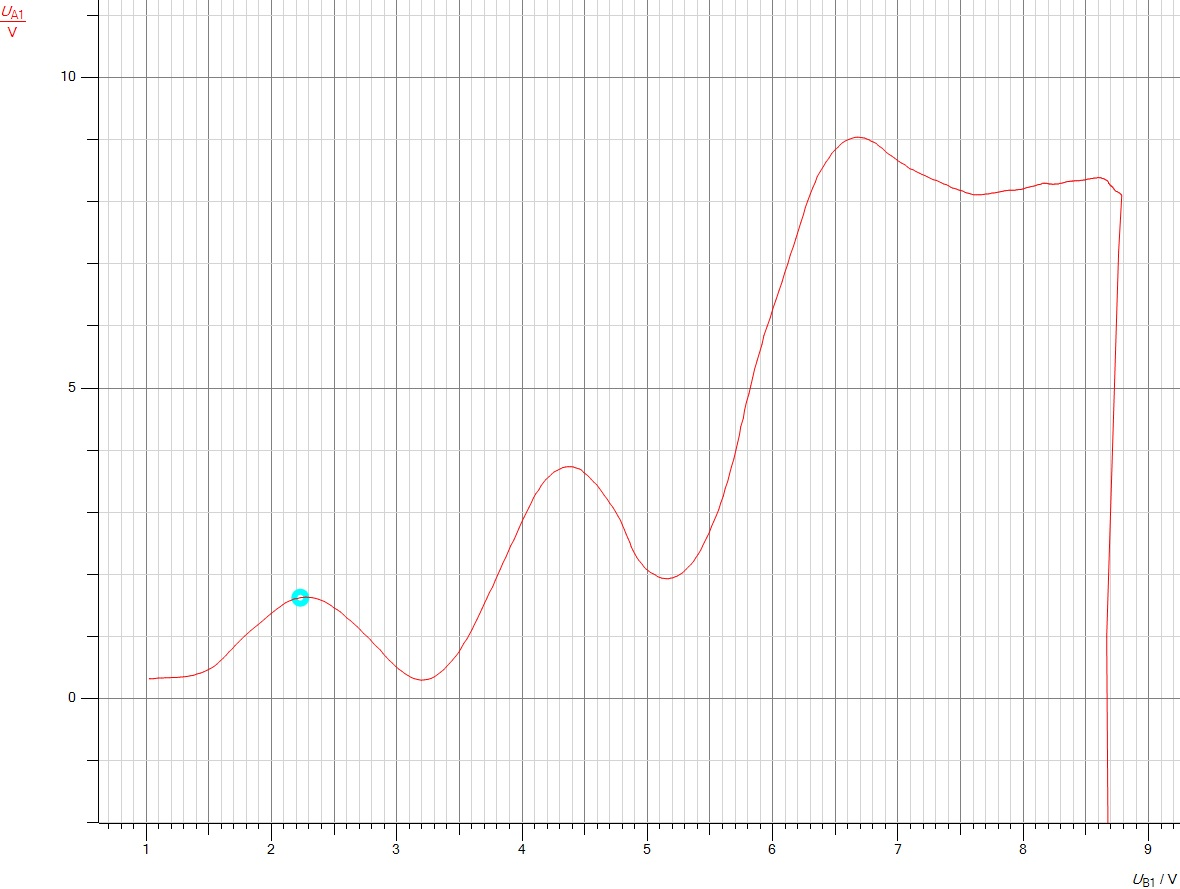
\includegraphics[scale=0.6]{Diagramm}\end{figure}
Es lässt sich erkennen, dass die Breite der Einbrüche nicht zu gering ist, was zunächst als Konflikt zur Theorie erscheinen kann, nach der ja nur ein präziser Energiewert der verschossenen Elektronen zu einem Einbruch führen kann. Dies lässt sich  aber durch verschiedene Faktoren erklären. Zum einen ist die Geschwindigkeit mit der die Elektronen auf das Neongas bei einer bestimmten Beschleunigungsspannung treffen nicht für alle Elektronen gleich, da die Elektronen mit unterschiedlichen Geschwindigkeiten aus dem Glühdraht treten und deshalb die Geschwindigkeit mit einer gewissen Verteilung (der Maxwell-Bolzmann Verteilung) auftritt.
Ein weiterer Faktor ist, dass aufgrund der thermischen Bewegung der Neonatome die entscheidende Relativgeschwindigkeit zwischen verschossenen Elektronen und Neonatomen nochmal einer zusätzlichen Verteilung unterliegt. Dieser Faktor lässt sich abschätzen durch die mittlere thermische Geschwindigkeit
\begin{equation*}\bar{v}=\sqrt{\frac{8k_B\,T}{\pi{m}}}\end{equation*}
für Neon erhalte ich eine mittlere Geschwindigkeit von $556.44\,\frac{m}{s}$ und für die Elektronen, die bei einer Glühtemperatur von $700\,K$ austreten, $1.6433\,10^{5}\,frac{m}{s}$. Da sich die Neonatome statistisch in jede Richtung bewegen, ist die maximale Geschwindigkeitsbandbreite durch die doppelte mittlere Geschwindigkeit der Neonatome zuzüglich der mittleren thermischen Energie der Elektronen gegeben. Wenn wir diese Geschwindigkeit von $1.6544\,10^{5}\,\frac{m}{s}$ in den entsprechenden Energieunterschied eines Elektrons über
\begin{equation*}E_\text{kin}=\left(\frac{1}{\sqrt{1-\left(\frac{v}{c}\right)^2}}-1\right)\,mc^2\end{equation*}
umrechnen, eine statistische Unschärfe von $0.077\,eV$. Zusätzlich zu diesem Phänomen kann das Elektron, bevor es einen inelastischen Stoß durchführt, mehrere elastische Stöße durchleben, die seine Energie verringern. Auch dadurch kommt noch ein zusätzlicher statistischer Anteil zur Geschwindigkeitsverteilung dazu. Dann kann es natürlich auch sein, dass ein verschossenes Elektron ein bereits angeregtes Neonatom stößt und weiter anregt. Durch dieses Vorgang erhält man Verringerungen der Intensität an unerwünschten stellen der Beschleunigungsspannung. Dieses Phänomen wurde während des Experiments gering gehalten, indem wir die Dichte des Gases sehr klein hielten.\newline
Neben diesen statistischen Verbreiterungen der Stromeinbrüche am Detektor, gibt es bei diesem Versuch auch systematische Fehler. Da Anode und Kathode aus unterschiedlichen Materialien bestehen, existiert zwischen ihnen eine gewisse Kontaktspannung, die der Beschleunigungsspannung entgegen steht. Des Weiteren verringern elastische Stöße auch die mittlere Energie der Elektronen, wodurch die Lage der Anregungsenergien verfälscht wird. Wie im Bild oben zu sehen ist, haben wir mehrere Einbrüche aufgezeichnet. Die Einbrüche bei höheren Spannungen kommen dadurch zustande, dass das Elektron genug Energie besitzt um zwei Neonatome anzuregen. Indem wir die Abstände zwischen diesen Einbrüchen messen, sollten wir immerhin die systematischen Fehler zu einem guten Teil eliminieren können. Wir bestimmten die Peakschwerpunkte der Einbrüche  sowie der Maxima unseres Messverlaufs auf folgende Werte
\begin{table}[H]\begin{tabular}{c | c}erster Einbruch&$3.204\pm0.652\,V$\\\hline
zweiter Einbruch&$5.25\pm0.634\,V$\\\hline
dritter Einbruch&$7.586\pm0.748\,V$\\\hline
erstes Maximum&$2.139\pm0.472\,V$\\\hline
zweites Maximum&$4.344\pm0.384\,V$\\\hline
drittes Maximum&$6.488\pm0.458\,V$
\end{tabular}\end{table}
Es muss beachtet werden, dass die vom Cassy Modul aufgezeichnete Spannung nur einem Zehntel der wirklichen Beschleunigungsspannung entspricht. Daraus berechnet sich dann die erste Anregungsenergie auf $21.83\pm3.97\,eV$. Wenn das Elektron des Neonatoms aus dem angeregten wieder in den Grundzustand übergeht, muss diese Energie über das Aussenden eines Photons der gleichen Energie abgegeben werden. Es bestimmt sich die Wellenlänge des emittierten Lichts auf $56.81\,nm$. Das können wir natürlich nicht sehen, da sichtbares Licht in einem Wellenlängenbereich von 450 bis 800 nm liegt, was einer Energie von $1.55\,eV$ bis $2.76\,eV$ entspricht. Im Experiment beobachtet man allerdings, dass das Gas dumpf orange leuchtet. Dies ist nun damit zu erklären, dass es Elektronen gibt die nicht in einem Anlauf, vom angeregten Zustand in den Grundzustand übergehen, sondern diesen Weg über Zwischenzustände gehen und somit mehrere Photonen geringerer Energie emittieren.

\section{Fazit}
Durch diesen Versuch konnte schön nochmal ein grundlegendes Verständnis eines vereinfachten Atomaufbaus und von Streuprozessen erworben werden. Außerdem konnte er eindrucksvoll die Diskretisierung der Energieniveaus im Atom zeigen, was seine historische Relevanz beglaubigt. Ich bin zufrieden mit unserem Ergebnis, das in einem plausiblen Bereich liegt.





\end{document}